\documentclass[11pt]{report}

\usepackage{graphicx}

\marginparwidth 0.5in 
\oddsidemargin 0.25in 
\evensidemargin 0.25in 
\marginparsep 0.25in
\topmargin 0.0in 
\textwidth 6in \textheight 8.5in

\title{HW3: Individual Contribution}
\author{bolt1003}

\begin{document}
\maketitle

\chapter{Application Domain Specification}

\subsection{User Profile Management (bolt1003)}
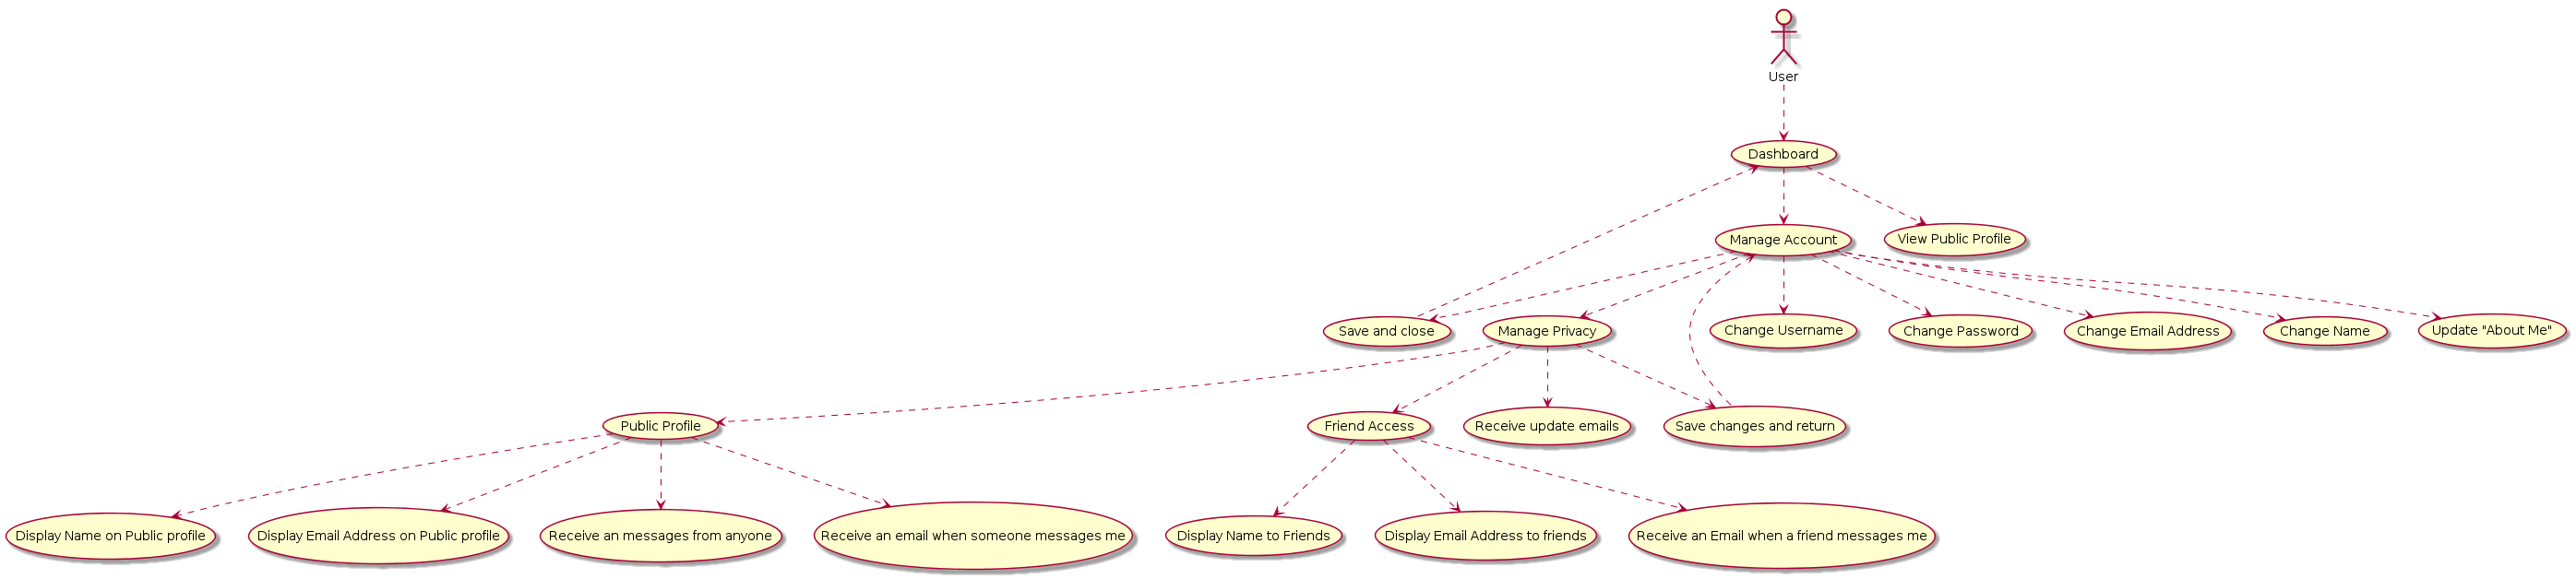
\includegraphics[width=\textwidth]{diagrams/bolt1003}

\section{Use Case Descriptions}

\subsection{Create Project from main menu(bolt1003)}
\begin{tabular}{ p{2cm} p{12cm} }
 \hline
 \\
 \textit{Actors:} & Users of sQuire. \\ 
 \\
 \textit{Goals:} & Create a Project. \\
 \\
 \textit{Pre-conditions:} & The user is logged in and at the bashboard. \\
 \\
 \textit{Summary:} & The user creates a project. \\ 
 \\
 \textit{Related use cases:} & None. \\ 
 \\
 \textit{Steps:} & \begin{enumerate}
  \item User selects the "+" icon and a wizard appears.
  \item A name is choosen for the project.
  \item Language is selected from a drop down menu.
  \item User clicks finish.
 \end{enumerate} \\
 \\
 \textit{Alternatives:} & Create project from the editor. \\
 \\
 \textit{Post-conditions:} & The user assigns permissions to access the project. \\
 \\
\hline
\end{tabular}

\subsection{Open a project (bolt1003)}
\begin{tabular}{ p{2cm} p{12cm} }
 \hline
 \\
 \textit{Actors:} & Users of sQuire. \\ 
 \\
 \textit{Goals:} & Choose the desired project and open it. \\
 \\
 \textit{Pre-conditions:} & One or more projects are available, the user is logged in and at the dashboard. \\
 \\
 \textit{Summary:} & User looks through a list of projects and selects the desired project. \\ 
 \\
 \textit{Related use cases:} & None. \\ 
 \\
 \textit{Steps:} & \begin{enumerate}
  \item User clicks on projects in the menu bar.
  \item A list of projects appears and the user clicks on the desired project.
 \end{enumerate} \\
 \\
 \textit{Alternatives:} & Open a project from recent projects. \\
 \\
 \textit{Post-conditions:} & User closes sQuire. \\
 \\
\hline
\end{tabular}








% Under Revision
% ################################################################################################


\subsection{Join Project (bolt1003)}
\begin{tabular}{ p{2cm} p{12cm} }
\hline
\\
\textit{Actors:} & Users of sQuire. \\ 
\\
\textit{Goals:} & Join an existing project.\\
\\
\textit{Pre-conditions:} & Must be registered, logged in and have permission to join a project.\\
\\
\textit{Summary:} & The user logs in, chooses a project, and joins the project. \\
\\
\textit{Related use cases:} & Invite user to project, Accept user invite. \\
\\
\textit{Steps:} & \begin{enumerate}
 \item The user selects a project.
 \item The user chooses the "Join". 
 \item The project is added to the users projects bar.
 \item The user selects the project and select "open".
\end{enumerate}\\
\\
\textit{Alternatives:} & User may decline an inventation to join a project. \\
\\
\textit{Post-conditions:} & You entered a Project. \\
\\
\hline
\end{tabular}






\subsection{Delete Project(mora5651)}
\begin{tabular}{ p{2cm} p{12cm} }
\hline
\\
\textit{Actors:} & User with permission.\\
\\
\textit{Goals:} & To delete an existing project. \\
\\
\textit{Pre-conditions:} & Must have permission to delete project. 
\\
\textit{Summary:} & Users are done with the project, and if the user has permission then they are allowed to delete the project. project is then deleted. \\
\\
\textit{Related use cases:} & Project Permissions. \\
\\
\textit{Steps:} & \begin{enumerate}
 \item The user clicks on the "Delete project" button. 
 \item A dialog is displayed. 
 \item User clicks either yes or no to delete project. 
 \item Project is then deleted. 
 \end{enumerate}\\
 \\
 \textit{Alternatives:} & User may choose not to delete the project in the confirmation display.\\
 \\
 \textit{Post-conditions:} & Deleted Project. \\
 \\
\hline
\end{tabular}

\subsection{Import File (Knic1468)}
\begin{tabular}{ p{2cm} p{12cm} }
\hline
\\
\textit{Actors:} & User with permission.\\
\\
\textit{Goals:} & To upload a file to the workspace. \\
\\
\textit{Pre-conditions:} & Must have permission to read/write. 
\\
\textit{Summary:} & User uploads a file into the workspace for collaborative editing. \\
\\
\textit{Related use cases:} & Project Permissions. \\
\\
\textit{Steps:} & \begin{enumerate}
 \item The user clicks on the "Import File" button. 
 \item System asks for a file to upload. 
 \item User picks a file to upload. 
 \item System reads file and uploads it into workspace. 
 \end{enumerate}\\
 \\
 \textit{Alternatives:} & System may reject a file if it is not the correct format.\\
 \\
 \textit{Post-conditions:} & None. \\
 \\
\hline
\end{tabular}

\subsection{Export Project(knic1468)}
\begin{tabular}{ p{2cm} p{12cm} }
\hline
\\
\textit{Actors:} & User with permission.\\
\\
\textit{Goals:} & To export a workspace to a local file. \\
\\
\textit{Pre-conditions:} & Must have read permission. 
\\
\textit{Summary:} & User saves a file to the local storage. \\
\\
\textit{Related use cases:} & Project Permissions. \\
\\
\textit{Steps:} & \begin{enumerate}
 \item The user clicks on the "Export File" button. 
 \item System promts the user to select a location and name. 
 \item User selects a file location. 
 \item System exports the file to the location. 
 \end{enumerate}\\
 \\
 \textit{Alternatives:} & System will display an error message of the location is write-protected.\\
 \\
 \textit{Post-conditions:} & None. \\
 \\
\hline
\end{tabular}

\subsection{Accept Invite to Project (carl7595)}
\begin{tabular}{ p{2cm} p{12cm} }   
 \hline
 \\
 \textit{Actors:} & User who received the invite (Invitee), sQuire user who sent the invite (Referrer), and Project Owner (Owner. May be the same as the Referrer). \\
 \\
 \textit{Goals:} & Gain access to a shared Project \\
 \\
 \textit{Pre-conditions:} & Authorized user with access to the project sends an email invite to another user. \\
 \\
 \textit{Summary:} & Access is granted to a project space using an invitation email. \\ 
 \\
 \textit{Related use cases:} & Create an account (if the invitee does not already have one), Login (if user is not logged in), and Create project (if the project has been deleted). \\
 \\
 \textit{Steps:} & \begin{enumerate}
  \item Invitee clicks on the link received by email.
	 \item New browser window opens with sQuire site.
	 \item Message appears that invitee's account has been added to the access list for the Project.
	 \item The project is added to their Projects list.
	 \item Owner and Referrer (who may be the same) receive an email informing them a new collaborator has been added
	 \item Project is opened in active pane of sQuire tab after a short delay.
	\end{enumerate} \\
 \\
 \textit{Alternatives:} & 2B. If invitee is not logged in to Squire, they are prompted for their credentials.
 
	2C. If invitee is does not have an Squire account, they are prompted to first create an account.
	
	3B. Project has been deleted. Invitee is informed the project does not exist and asks if they would like to create a new project with that name.
	
	3C. Join link has been deactivated because of previous use/time limit. Invitee is informed that the invite has expired and is no longer valid, instructing them to contact the Project Owner for access. \\
 \\
 \textit{Post-conditions:} & Invitee has been added to Project access list. Invite link is deactivated to prevent mulitple joins off of old links. Owner has been notified of new collaborator. \\
 \\
\hline
\end{tabular}

\subsection{Remove User to Project (carl7595)}
\begin{tabular}{ p{2cm} p{12cm} }   
 \hline
 \\
 \textit{Actors:} & sQuire user with access to the Project (Member), Authorized user who requests the removal (Agent), and Owner of the Project (Owner. May be the same as the Agent) \\
 \\
 \textit{Goals:} & Revoke access to the Project for a single or multuple users. \\
 \\
 \textit{Pre-conditions:} & Agent has permission to edit the Project access list, and agent is logged into Squire and has opened this Project. \\
 \\
 \textit{Summary:} & One or more user accounts are removed from the access list for a Project. \\ 
 \\
 \textit{Related use cases:} & None.  \\ 
 \\
 \textit{Steps:} & \begin{enumerate}
  \item Agent selects the access list for this Project.
	 \item Agent selects an account (or multiple accounts) and selects "Remove from Project".
	 \item Agent is prompted for confirmation, and selects 'Yes'.
	 \item The access list is modified to remove the selected account(s).
	 \item Owner and Member(s) receive an email informing of the change of access.
	 \item Member's Project lists are updated to no longer display the Project.
	 \item Member's Project panes related to this Project forced to close on next refresh.
 \end{enumerate} \\
 \\
 \textit{Alternatives:} & \begin{itemize} 
	 \item 2B. Agent does not have correct permissions. Error messsage informs them that they cannot edit Project access list.
	 \item 3B. Agent clicks 'No'. Access list is not modified.
	\end{itemize}\\
 \\
 \textit{Post-conditions:} & \begin{itemize}
	 \item Members have been removed from the Project, and their client windows closed to prevent continued access.
	 \item Owner and Member have been notified of the change.
 \end{itemize}\\
 \\
\hline
\end{tabular}

\subsection{Edit Project Permissions (benz5834)}
\begin{tabular}{ p{2cm} p{12cm} }
 \hline
 \\
 \textit{Actors:} & Squire user \\ 
 \\
 \textit{Goals:} & Edit the permissions for a project \\
 \\
 \textit{Pre-conditions:} & User must have the project that he wants to edit the permissions of open. \\
 \\
 \textit{Summary:} & User opens up the settings menu and navigates to permissions, adds (or removes) users individual access rights to the project.  \\ 
 \\
 \textit{Related use cases:} & Add user to project, Remove user from project. \\ 
 \\
 \textit{Steps:} & \begin{enumerate}
  \item Click the settings button in project.
  \item System opens settings menu.
  \item User clicks permissions link.
  \item System opens the permissions menu.
  \item User selects user from list of users.
  \item User adds read or write permissions to user.
  \item User saves changes and exits permissions.
 \end{enumerate} \\
 \\
 \textit{Alternatives:} & User can remove read or write permission instead in step 6. User can discard changes instead in step 7. \\
 \\
 \textit{Post-conditions:} & None. \\
 \\
\hline
\end{tabular}

\end{document}